\chapter{Mathematisch-formale Beschreibung des Problems}
Aus einer Sequenz von Objekten sollen alle Duplikate entfernt werden. Ein Objekt besteht dabei aus einem Schlüssel eines uniformen Typs und eventuell einem Wert. 

Mathematisch betrachtet, ist die gegebene Sequenz eine partielle Multifunktion \(s: K\multimap{W}\), die eine Menge von Schlüsseln \(K\) auf eine Menge von Werten \(W\) abbildet. Dabei können einem Element des Definitionsbereiches mehrere Elemente des Wertebereiches zugeordnet werden. Ziel ist es die Korrespondenz der Mengen \(K\) und \(W\) zu entfernen, indem eine partielle Funktion \(s': K\to{W}\) bestimmt wird. Wird in \(s\) ein Schlüssel \(k\in{K}\) mehreren Werten \(w_{0}, \dots{}, w_{n}\in{W}\) zugeordnet, so soll in \(s'\) jenes Paar \((k, w_{i})\) übernommen werden, welches das größte \(w_{i}\in{w_{0}, \dots{}, w_{n}}\) bezüglich einer gegebenen, totalen Ordnung \(\le\) enthält.

Partielle Abbildungen zwischen zwei Mengen werden durch den abstrakten Datentypen Wörterbuch modelliert. Zu konkreten Datentypen, die diesen Datentypen implementieren, zählen beispielsweise Listen, Suchbäume und Hash-Tabellen. Diese Arbeit verfolgt das Ziel, das Problem mit Hilfe von Hash-Tabellen zu lösen. Die Motivation von Hash-Tabellen ist es, die Operationen auf die Datensätze durch direkten Zugriff umzusetzen, wodurch sich der Datentyp eignet, um Problem zu lösen, bei denen die Laufzeit relevant ist.

\chapter{Anwendungsszenario}
Als Anwendungsfall soll der Algorithmus pcap-Dateien verarbeiten. In einer pcap-Datei (packet capture) können alle Pakete gespeichert werden, die in einem festen Zeitraum innerhalb eines Netzwerks verschickt wurden. Zu den gespeicherten Paketdaten gehören beispielsweise die MAC-Adresse von Sender und Empfänger des Paketes, was die Analyse des Verkehrs in Netzwerken ermöglicht. 

Konkret soll das Programm eine pcap-Datei einlesen und für jedes Paket die MAC-Adresse des Senders zur Hash-Tabelle hinzufügen. Der Wert zu einer entsprechenden MAC-Adresse soll beginnend bei dem Wert 1 inkrementell bei jedem erneuten Aufkommen der gleichen MAC-Adresse erhöht werden. Das Ergebnis ist eine Hash-Tabelle in der die MAC-Adressen aller Geräte gespeichert sind, die im Zeitraum zur Aufnahme der pcap-Datei mindestens ein Paket versendet haben. 

Angenommen in einem industriellen Netzwerk wird jeden Tag zu festgelegten Zeiten der Verkehr im Netzwerk mit einer pcap-Datei aus Sicherheitsgründen aufgenommen, so kann durch das Programm festgestellt werden, ob en dem Netzwerk ein potentieller Eindringling aufgetaucht ist oder etwa von einem Gerät fälschlicherweise Pakete versendet wurden.

Die Paketdaten, welche in pcap-Dateien gespeichert werden, bieten weitaus mehr Informationen, wie zum Beispiel das Protokoll, mit dem das entsprechende Paket versendet wurde, was dem Algorithmus Raum zur Erweiterung lässt. Als Testdaten können entsprechende Dateien synthetisch hergestellt werden. Des Weiteren existieren frei verfügbare pcap-Dateien aus der Realität, die von verschiedenen Organisationen bereitgestellt werden.

\chapter{Beschreibung und Implementierung des Algorithmus}
\section{Vorbetrachtung und Beschreibung}
Hash-Tabelle, welche für das Programm implementiert werden, unterstützen folgende Operationen:
\begin{itemize}	
	\item Einfügen(k,v): Der Datensatz (k,v) wird in die Datenstruktur aufgenommen, sofern \(k\notin{R}\) gilt, andernfalls geschieht nichts.
	\item Entfernen(k): Falls ein Datensatz (k,v) in der Datenstruktur existiert, wird dieser aus der Datenstruktur entfernt, andernfalls geschieht nichts.
	\item Suchen(k): Gibt einen Wahrheitswert aus, der wahr ist, falls ein Datensatz (k,v) in der Datenstruktur existiert und falsch sonst.
\end{itemize}
Dabei werden für dieses Problem lediglich dich Operationen \textit{Einfügen} und \textit{Suchen} benötigt. Die Eingabedaten werden schrittweise ausgelesen und dabei wird bei jedem Objekt geprüft, ob sich dieses bereits in der Hash-Tabelle befindet. Ist es nicht in der Hash-Tabelle, so wird das Objekt in die Hash-Tabelle eingefügt. Andernfalls, wird der zum entsprechenden Schlüssel gehörige Wert inkrementiert. 
\newpage
In Pseudo-Code sieht das Vorgehen folgendermaßen aus:
\begin{lstlisting} [caption={Einfügen der Eingabedaten in die Hash-Tabelle}]
REMOVE-DUPLICATES(Eingabe input):
  ht = HashTable()
  for (k, v) in input:
      if ht.contains(k):
          ht[k] = ht[k] + 1
      else:
          ht.insert((k,v))
  return ht
\end{lstlisting}
Da in jedem Fall alle Elemente aus der Eingabesequenz betrachtet werden müssen, ist die Laufzeit voraussichtlich von der Anzahl eingelesener Element sowie der benötigten Laufzeit für die Operationen Suchen und Einfügen abhängig. Bei \(n\) zu bearbeitenden Elementen wird in jedem Fall \(n\) mal die Such-Operation ausgeführt. Wie oft eingefügt wird ist von der Anzahl Duplikate abhängig. 

Da das Einfügen aus Sicht der Laufzeit teurer als das inkrementieren eines Wertes ist, ist die worst-case Eingabe eine Sequenz ohne Duplikate. Für das Anwendungsszenario mit realen Daten wird dieser Fall niemals eintreten, sondern stattdessen die Anzahl von Duplikaten den Großteil der Eingabesequenz ausmachen. Aus diesem Grund ist ein Hash-Verfahren angebracht, bei dem mit konstanter Laufzeit gesucht wird. Da dies bei üblichen Verfahren, wie dem Doppel-Hashing oder etwa dem Chaining im worst-case nicht der Fall ist, wird das Kuckucks-Hashing verwendet.

Beim Kuckucks-Hashing werden zwei Hash-Tabellen \(T_{1}\) und \(T_{2}\) der Länge \(m\) mit zwei Hash-Funktionen \(h_{1}\) und \(h_{2}\) benutzt werden. Für jeden Schlüssel \(x\) gilt entweder \(T_{1}[h_{1}(x)]=x\) oder \(T_{2}[h_{2}(x)]=x\). Demnach werden beim Suchen maximal zwei Hash-Adressen abgeprüft, was zu einer konstanten Laufzeit sogar beim worst-case führt.

Das Verhalten beim Einfügen ist, was dieser Variante ihren Namen gibt: beginnend bei der ersten Hash-Tabelle wird der entsprechende Datensatz versucht einzufügen. Kommt es zu einer Kollision, wird der Schlüssel, der die entsprechende Hash-Adresse belegt, in die zweite Hash-Tabelle verdrängt. Auf diese Weise werden nacheinander Schlüssel zwischen den Hash-Tabellen verschoben, bis kollisionsfrei eingefügt werden kann. Da bei diesem Verfahren Endlosschleifen auftreten können ist die Anzahl der Verschiebungen auf \(\lfloor \log{m}\rfloor\) begrenzt. Wird dieser Wert erreicht, so wird ein Re-Hashing durchgeführt und danach der Schlüssel erneut eingefügt.

Ein Re-Hashing mit vergrößern der Hash-Tabelle wird außerdem durchgeführt, wenn die Hash-Tabelle den Füllgrad \(0,5\) überschreitet, da bis zu diesem Schwellenwert das Einfügen eine amortisiert konstante Laufzeit benötigt. Es hat sich herausgestellt, dass die Wahl der Hash-Funktionen, der Größe der Hash-Tabellen, der Vergrößerung beim Re-Hashing, dem maxmialen Füllgrad und der maximal erlaubten Schleifendurchläufe beim Einfügen die Laufzeit des Algorithmus beeinflussen. Im Laufe der Untersuchung der Laufzeit wurde des Weiteren eine Variante des Kuckucks-Hashing mit Buckets und einem Stash zum Vergleich implementiert. Mehr dazu im letzten Kapitel. 

\section{Implementierung des Kuckucks-Hashing}
Der Algorithmus wurde mit der Programmiersprache Python umgesetzt. Konkreter Python2, da die Bibliothek Scapy, welche für das Arbeiten mit pcap-Dateien benötigt wird, Python3 nicht unterstützt. Da mehrere Varianten des Hashings implementiert werden, wurde zunächst eine Schnittstelle in Form einer abstrakten Klasse angelegt, um das gewünschte Verhalten näher zu spezifizieren.
\newpage
\begin{lstlisting} [caption={Abstrakte Klasse für Hash-Tabellen}]
import abc
from collections import namedtuple

class HashTable(object):
    __metaclass__ = abc.ABCMeta
    entry = namedtuple("entry", ["key", "value"])
    bottom = entry(None, None)

@abc.abstractmethod
def insert(self, key, value):
    pass

@abc.abstractmethod
def contains(self, key):
    pass

@abc.abstractmethod
def entries(self):
    pass
\end{lstlisting}
Dabei dient \(insert\) dem Einfügen eines Datensatzes, \(contains\) liefert einen Wahrheitswert über die Anwesenheit eines Schlüssels und \(entries\) gibt einen Generator mit allen Datensätzen der Hash-Tabelle aus. Die einzelnen Datensätze werden durch das benannte Tupel \(entry\) umgesetzt, welches der besseren Leserlichkeit im Code dient verglichen zu Verschachtelten Index-Zugriffen auf klassischen Tupeln in Listen.
\newpage
Der Konstruktor für die Klasse, welche das normale Kuckucks-Hashing implementiert ist folgender:
\begin{lstlisting} [caption={Konstruktor der Klasse Cuckoo-Hash}]
class CuckooHash(HashTable):
    def __init__(self, size):
        self.size = size
        self._elementcount = 0
        self._maxloop = int(log(size))
        self._table1 = [None] * size
        self._table2 = [None] * size
        self._hf1 = universal_hash(size)
        self._hf2 = universal_hash(size)
\end{lstlisting}
Die Instantiierung erwartet die Größe der Hash-Tabellen \textit{size}, mit der zwei leere Hash-Tabellen initialisiert werden. Da es in Python keine Arrays mit statischer Größe gibt, werden diese hier mit Listen simuliert. Der Standardwert für ein Feld ist dabei \textit{None}, damit später die Auswertung beim Index-Zugriff auf ein leeres Feld als Bedingung in einer if-Anweisung als falsch ausgewertet wird. Mit welcher Funktion die beiden Hash-Funktionen generiert werden, wird an einem später Punkt erklärt. Eine Instanz von \textit{CuckHash} besitzt außerdem die Attribute \textit{elementcount} zur Berechnung des Füllgrades und \textit{maxloop} als Begrenzung für die maximalen Schleifendurchläufe beim Einfügen.

Die Operation \textit{contains} ist beim Kuckucks-Hashing simpel, da sich ein Datensatz mit einem gesuchten Schlüssel lediglich an zwei Positionen befinden kann:
\begin{lstlisting} [caption={Implementierung von contains}]
def contains(self, key):
	return (self._table1[self._hf1(key)] and self._table1[self._hf1(key)].key) 
	       or (self._table2[self._hf2(key)] and self._table2[self._hf2(key)].key)
\end{lstlisting}
Dabei erfüllt die kompakte Schreibweise den Zweck, dass bei Auswertung des ersten Arguments der \textit{or}-Anweisung als wahr, das zweite Argument nicht ausgewertet wird, womit unnötige Operationen eingespart werden.

Das Einfügen beim Kuckucks-Hashing ist im Vergleich komplexer und wurde folgendermaßen umgesetzt:
\begin{lstlisting} [caption={Implementierung von insert}]
def insert(self, key, value):
    for _ in range(self._maxloop):
        hashaddr = self._hf1(key)
        if self._table1[hashaddr]:
            oldentry1 = self._table1[hashaddr]
            self._table1[hashaddr] = self.entry(key, value)
        else:
            self._table1[hashaddr] = self.entry(key, value)
            self._ckeck_for_rehash_and_resize()
            return

        hashaddr = self._hf2(oldentry1.key)
        if self._table2[hashaddr]:
            key = self._table2[hashaddr].key
            value = self._table2[hashaddr].value
            self._table2[hashaddr] = oldentry1
        else:
            self._table2[hashaddr] = oldentry1
            self._ckeck_for_rehash_and_resize()
            return

    self._rehash()
    self.insert(key, value)
\end{lstlisting}
Hier wird maximal \textit{maxloop} mal nacheinander in die Hash-Tabellen \textit{table1} und \textit{table2} eingefügt. Ist ein kollisionsfreies Einfügen möglich, so wird mit \textit{ckeck\_for\_rehash\_and\_resize} geprüft, ob ein Re-Hashing mit Vergrößern der Hash-Tabellen durchgeführt werden muss. Tritt beim Einfügen eine Kollision auf, so wird der verdrängte Datensatz in die nächste Hash-Tabelle eingefügt. Falls die Schleife beendet wird, so wird ein Re-Hashing durchgeführt und danach die Einfüge-Operation erneut ausgeführt.

Beim Re-Hashing werden alle Datensätze, die sich in beiden Hash-Tabellen befinden, gesammelt und in leere Hash-Tabellen mit neuen Hash-Funktionen erneut eingefügt:
\begin{lstlisting} [caption={Implementierung von rehash}]
def _rehash(self):
    ht1 = (entry for entry in self._table1 if entry)
    ht2 = (entry for entry in self._table2 if entry)
    self._reset()

    for entry in chain(ht1, ht2):
        self.insert(entry.key, entry.value)
\end{lstlisting}
Das Erstellen leerer Hash-Tabellen und Generieren neuer Hash-Funktionen wird dabei durch die \textit{reset}-Funktion übernommen. Die verwendeten Hash-Funktionen werden zufällig aus einer Familie von universalen Hash-Funktionen gewählt:
\begin{lstlisting} [caption={Generierung der Hash-Funktionen}]
def universal_hash(m):
    p = next_prime(m)
    a = randint(2, p - 1)
    b = randint(1, p - 1)
    return lambda x: ((a * x + b) % p) & (m-1)
\end{lstlisting}
Dabei ist \textit{m} die aktuelle Größe der Hash-Tabelle, \textit{p} eine Primzahl, die größer als \textit{m} ist und \textit{a} und \textit{b} sind zwei Zufallszahlen kleiner als \textit{p}. Die Implementierung der Funktion \textit{next\_prime} bietet dabei viel Spielraum für Optimierungen, welche im letzten Kapitel näher betrachtet werden. Das Ziel von universalen Hash-Funktionen ist es, dass zwei zufällig gewählte Schlüssel eine Chance von \(1/m\) haben zu kollidieren. Des Weiteren soll es möglich sein zufällige Hash-Funktionen zu generieren, um flexibles Re-Hashing zu ermöglichen.

\chapter{Messung der Laufzeiten}
\section{Laufzeitmessung mit synthetischen Eingabedaten}
Für die ersten Laufzeitmessungen wurden mit einem Benchmark Sequenzen von Integern generiert. Als Probleminstanzen wurden dabei \(2, 4, \dots{}, 10\) Millionen Integern pro Datei verwendet und wiederum pro Probleminstanz 20 verschiedene Dateien generiert. Die Integer befinden sich zunächst in dem Intervall \([1, 256]\), um anfangs das Verhalten der Hash-Tabelle bei vielen Kollisionen zu prüfen, was dem Anwendungsszenario nahe kommt. Pro Datei wurde der Algorithmus drei mal ausgeführt und bei jedem Durchlauf die Laufzeit gemessen. Für jeden Probleminstanz wurden danach die Standardabweichung und der Mittelwert aus alle zugehörigen Laufzeiten bestimmt.
\newpage
Die Funktion zur Zeitmessung definiert einen Dekorator, welcher über die Deklaration jeder Funktion geschrieben werden kann, deren Zeit gemessen werden soll:
\begin{lstlisting} [caption={Dekorator für Zeitmessung}]
from functools import wraps
from time import time

def timer(func):
    @wraps(func)
    def wrapper(*args, **kwargs):
        start = time()
        func(*args, **kwargs)
        end = time()
        return end-start
    return wrapper
\end{lstlisting}
Für die Messung selbst wird das Modul \textit{time} verwendet, welches unter Linux eine ausreichende Präzision bieten sollte.
Die Messungen ergeben folgende Werte:
\newpage
\begin{figure}[H]
	\hspace*{-1.7cm}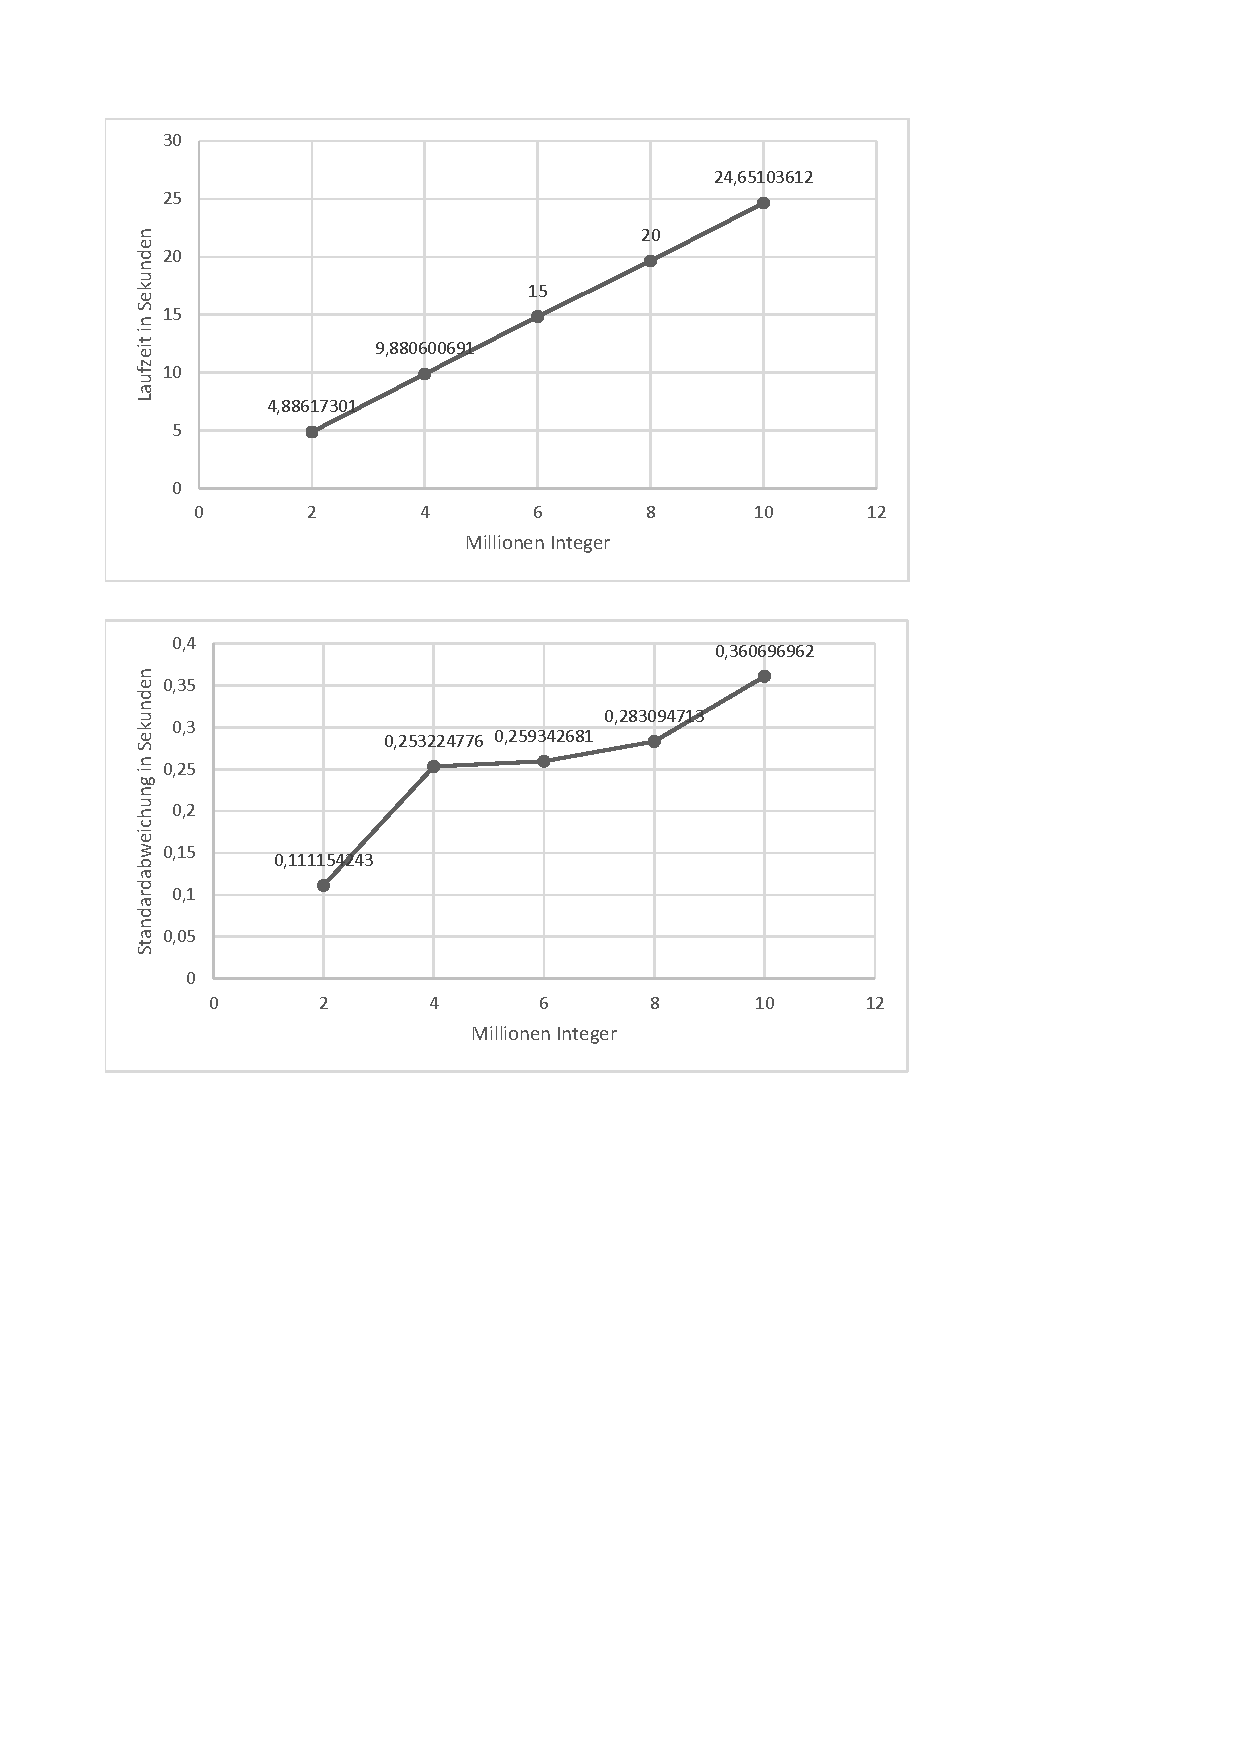
\includegraphics[width=1.5\linewidth]{Bilder/benchmark_2M.pdf}
\end{figure}
\newpage
Die durchschnittliche Laufzeit (in der oberen Grafik dargestellt) zeigt ein lineares Wachstum. Bei lediglich 256 verschiedenen Integern, die vorkommen können, muss pro Durchlauf mit einer Startgröße von 64 für die Hash-Tabellen genau drei mal ein Re-Hashing durchgeführt werden. Das ist für eine Hash-Tabelle relativ wenig, wodurch die Laufzeit zum Großteil aus dem Ausführen von \textit{contains}-Operationen besteht. Daher entsteht eine lineare Abhängigkeit. Die untere Grafik zeigt die Standardabweichung für jede Probleminstanz, die vernachlässigbar gering ist.

Als nächstes werden Laufzeitmessungen mit synthetisierten Eingabesequenzen, die aus MAC-Adressen bestehen, durchgeführt. Ziel dieser Messungen ist es, den Einfluss des Re-Hashing auf die Laufzeit zu ermitteln und die Eingabe-Daten an das Anwendungsszenario anzupassen. Das Unternehmen Cisco klassifiziert Netzwerke nach Anzahl der Geräte wie folgt: ein kleines Netzwerk hat bis zu 200 Gerät, ein mittleres bis zu 1000 und ein großes mehr als 1000. Beginnend bei kleinen Netzwerke, werden erneut die Probleminstanzen \(2, 4, \dots{}, 10\) Millionen MAC-Adressen pro Datei verwendet. Es werden erneut 10 Dateien pro Probleminstanz generiert, die zunächst aus maximal 256 verschiedene MAC-Adressen. Somit ist das Ergebnis mit den gemessenen Laufzeiten für Integer bis 256 vergleichbar. Die Laufzeitmessungen für kleine Netzwerke haben Folgendes ergeben:
\newpage
\begin{figure}[H]
	\hspace*{-1.7cm}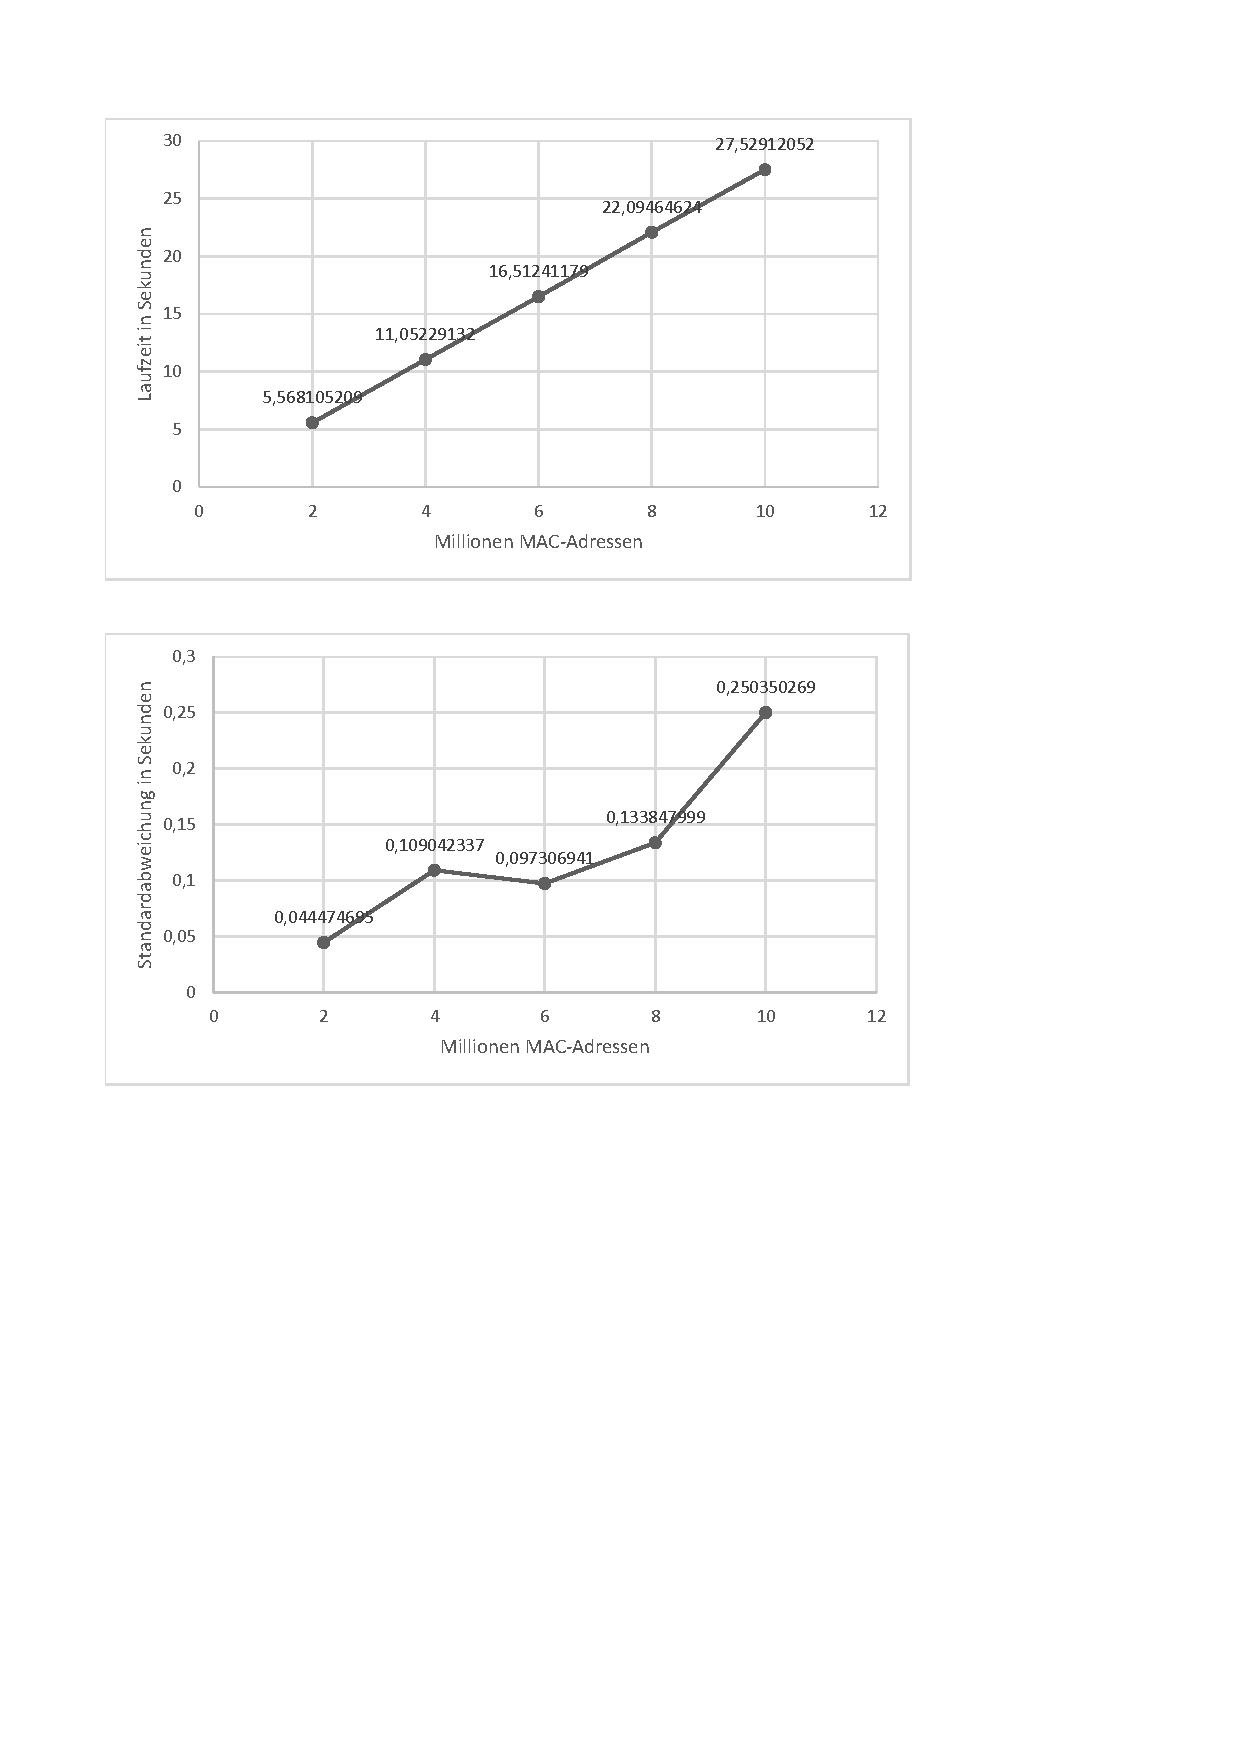
\includegraphics[width=1.5\linewidth]{Bilder/benchmark_network_small.pdf}
\end{figure}
\newpage
Die durchschnittlichen Laufzeiten für die verschiedenen Probleminstanzen im oberen Graphen zeigen eine ähnlich lineare Tendenz wie beim ersten Testfall. Dabei sind die Laufzeiten stets ungefähr 2 Sekunden höher. Ein Grund dafür könnte sein, dass die MAC-Adressen in Integer konvertiert werden, die beträchtlich größer als die Integer bis 256 sind, wodurch die Rechenoperationen mehr Zeit benötigen. Im zweiten Graphen wird die Standardabweichung dargestellt, die auch hier vernachlässigbar gering ist.

Bei den Laufzeitmessungen für Netzwerke mittlerer Größe wurden die Anzahl verschiedener MAC-Adressen auf 512 erhöht. In Anbetracht der vergleichsweise hohen Anzahl an MAC-Adressen wird diese Änderung vermutlich keine großen Auswirkungen auf das Ergebnis haben. Die Laufzeitmessungen für mittlere Netzwerke sind in den folgenden Graphen dargestellt:
\begin{figure}[H]
	\hspace*{-1.7cm}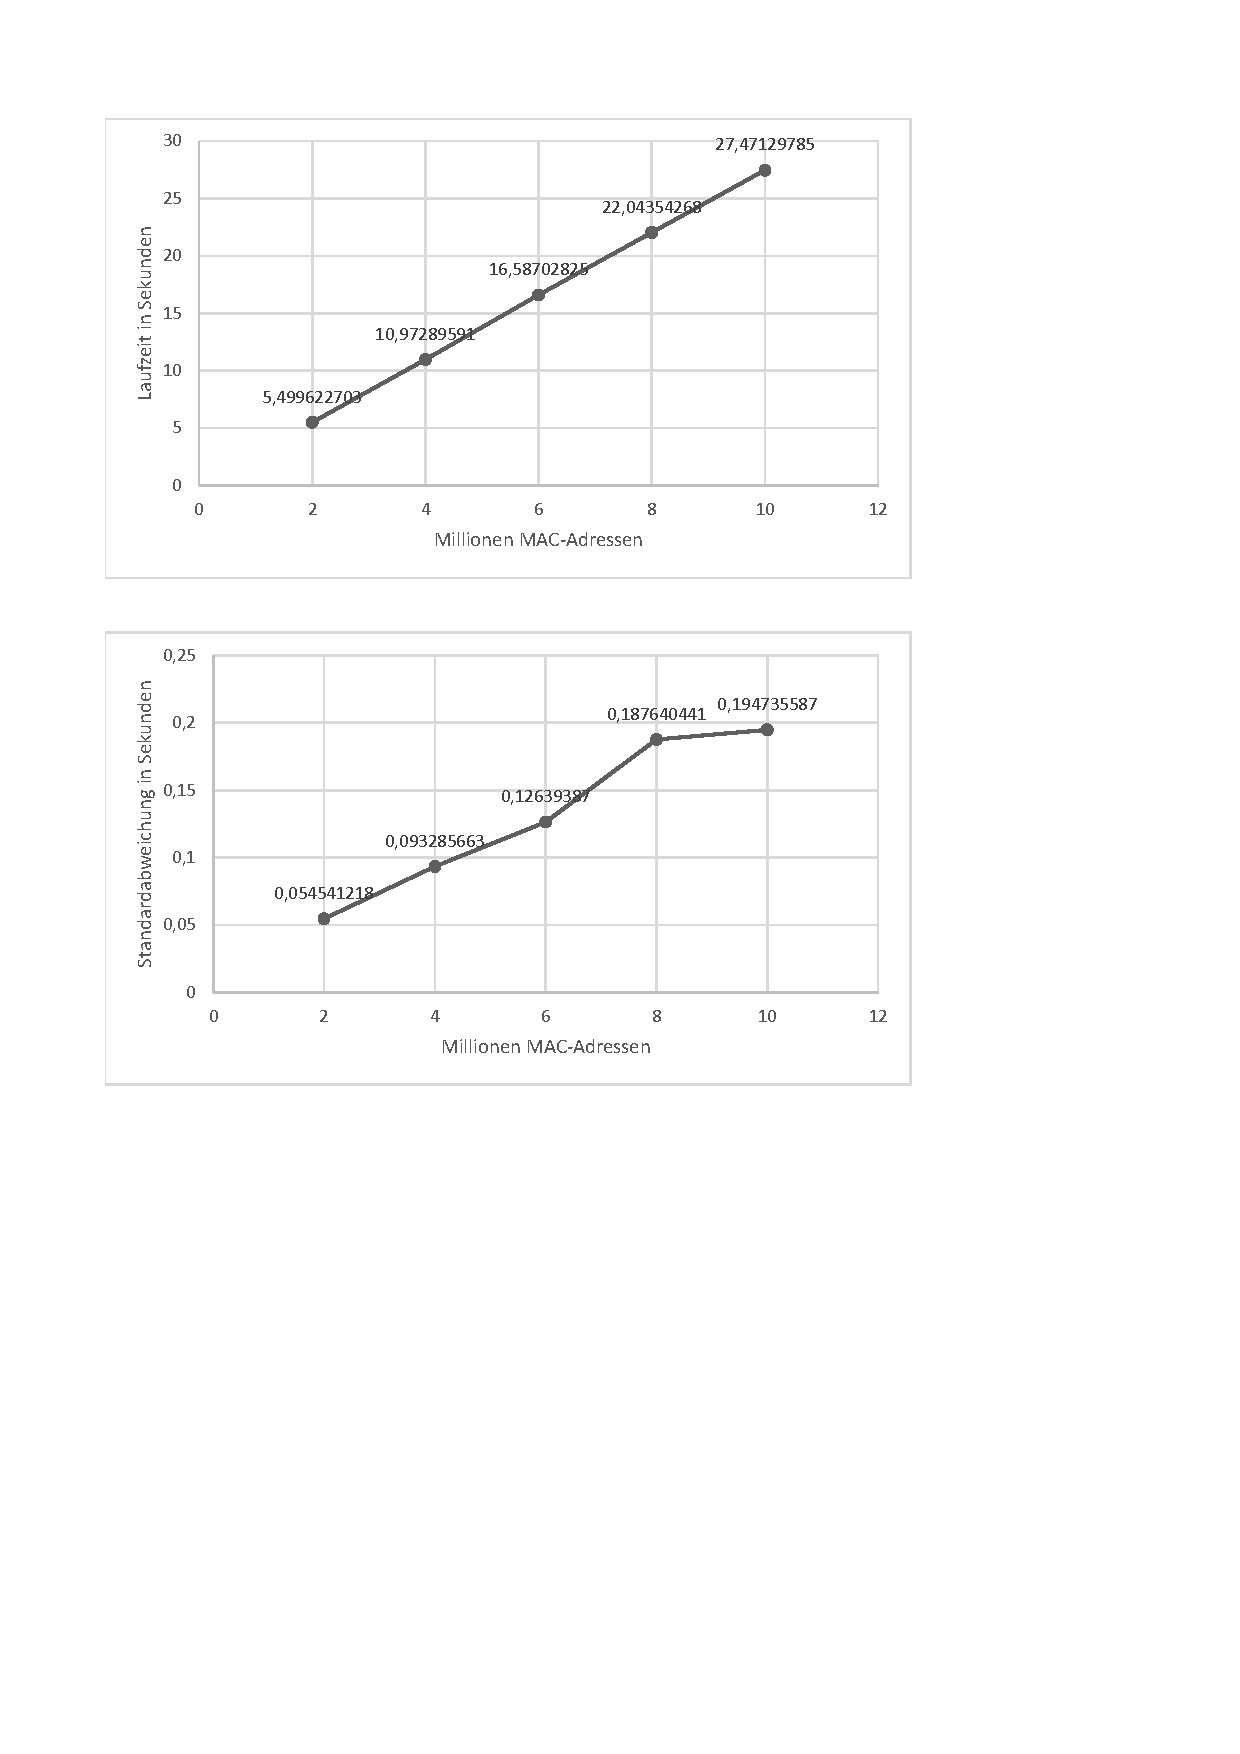
\includegraphics[width=1.5\linewidth]{Bilder/benchmark_network_medium.pdf}
\end{figure}
\newpage
Obwohl für jede Probleminstanz ein Re-Hashing mit Vergrößerung mehr benötigt wird, zeigt der obere Graph, dass die durchschnittlichen Laufzeiten beinahe gleich, wie die der kleinen Netzwerke, sind. Für die durchschnittlichen Laufzeiten und die Standardabweichung gelten daher die gleichen Beobachtungen. 

Für den Testfall für große Netzwerke wurde die Anzahl der verschiedenen MAC-Adressen auf 2048 erhöht, was zu dem nachstehenden Ergebnissen führt:
\begin{figure}[H]
	\hspace*{-1.7cm}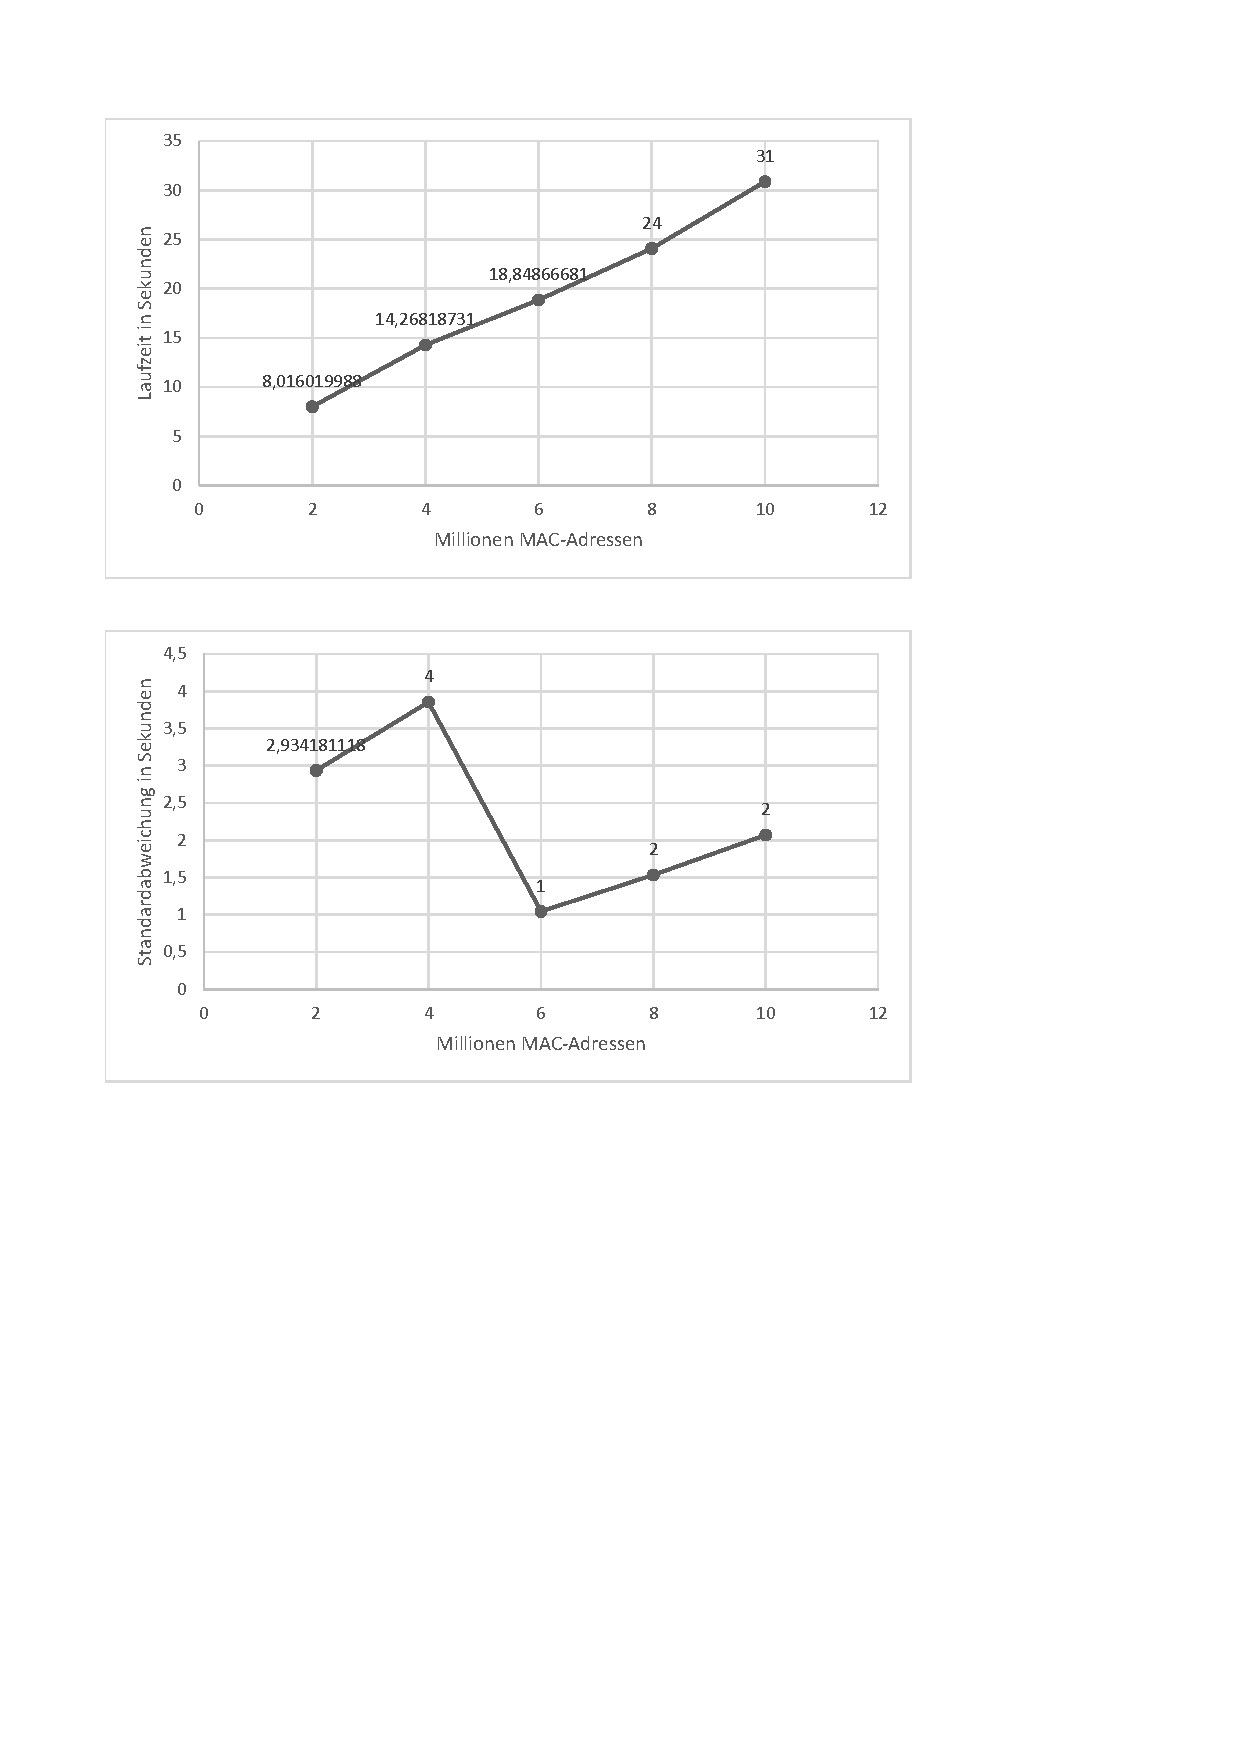
\includegraphics[width=1.5\linewidth]{Bilder/benchmark_network_large.pdf}
\end{figure}
\newpage
Das Ergebnis zeigt einen großen Unterschied zu den vorherigen Laufzeitmessungen. Für alle Probleminstanzen sind die im zweiten Graphen dargestellten Standardabweichungen vergleichsweise sehr hoch. Bei den Eingabedaten sind erstmals Re-Hashings wegen überschreiten des maximalen Schleifenwertes beim Einfügen aufgetreten. Wie oft dies der Fall war, hing von den entsprechenden Eingabedaten ab, weswegen die hohen Standardabweichungen entstehen.

Des Weiteren scheint die lineare Entwicklung der durchschnittlichen Laufzeiten in dem ersten Graphen nur noch für die letzten drei Probleminstanzen gültig zu sein. Bei den Probleminstanzen mit 2 und 4 Millionen MAC-Adressen liegen die ermittelten Laufzeiten klar über der linearen Tendenz. 

Theoretisch besteht die Laufzeit \(T\) aller gemessen Fälle stets aus zwei Teilen \(v\) und \(d\), womit gilt \(T=v+d\). Dabei beschreibt \(v\) die Zeit die für das tatsächliche Einfügen verwendet wird. Also für große Netzwerke das Einfügen von \(2048\) MAC-Adressen. Die Laufzeit \(d\) beschreibt dann die Zeit die benötigt wird, um die \textit{contains}-Operation auf alle übrigen Duplikate anzuwenden. In den gemessenen Testfällen und dem Anwendungsszenario wird die Menge der verschiedenen Elemente stets viel kleiner als die Gesamtmenge der eingegebenen Elemente sein. Die Anzahl der Duplikate ist demnach sehr hoch. In den ersten beiden Probleminstanzen hat der Schwellwert \(v\) noch einen größeren Einfluss auf \(T\), weswegen \(T\) über der linearen Tendenz liegt.

\section{Laufzeitmessung mit realen Eingabedaten}
Für die Messungen wurden in der Realität aufgenommene pcap-Dateien verwendet, die in einem Versuchslabor der cyber security Konferenz 4SICS aufgenommen wurden. Es wurden drei pcap-Dateien jeweils 10 mal analysiert und die durchschnittliche Laufzeit sowie die Standardabweichung bestimmt. Die verschiedenen Dateien hatten folgende Eigenschaften:
\begin{table}[H]
	\centering
	\begin{tabular}{|c|c|c|}
		\hline
		Testfall & Anzahl Pakete & Anzahl Geräte \\ \hline
		No. 1 & 246137 & 9 \\
		No. 2 & 1253100 & 36 \\
		No. 3 & 2274747 & 54 \\ \hline
	\end{tabular}
	\caption{Testfälle für Laufzeitmessungen mit realen Daten}
\end{table}
Die Dateien wurden mit der Bibliothek \textit{scapy} paketweise ausgelesen. Aus den Paketen wurde die MAC-Adresse des Absenders extrahiert und danach wie gewohnt der Algorithmus angewendet. Dabei wurden die gesamte Laufzeit des Programmes und der Anteil dieser Laufzeit, der durch Operationen auf der Hash-Tabelle verbraucht wurde, gemessen. Es entstnaden folgende Messdaten:
\begin{table}[H]
	\centering
	\begin{tabular}{|c|c|c|}
		\hline
		Testfall & durchsch. Laufzeit & durchschn. Laufzeit Operationen Hash-Tabelle \\ \hline
		No. 1 & 148,9871 s & 4,019 s \\
		No. 2 & 741,651 s & 20,6029 s \\
		No. 3 & 1291,329 s & 37,0405 s \\ \hline
	\end{tabular}
	\caption{Messdaten für Laufzeitmessungen mit realen Daten}
\end{table}
Die Daten zeigen, dass das Auslesen der pcap-Dateien selbst viel Zeit in Anspruch nimmt. Würden für die Laufzeitmessungen größere Dateien verwendet werden, die für die Optimierung der Datenstruktur interessanter sind, wären die Laufzeiten nicht mehr vertretbar. Aus diesem Grund wurden für die Analyse der Implementierungen weiterhin synthetische Daten verwendet. 

In Anbetracht der gemessenen Laufzeiten, die nur durch Operationen auf der Hash-Tabellen entstanden, lassen sich diese grob in den Trend einordnen, der bereits in den vorherigen Tests beobachtet wurde. Eine erhöhte Anzahl von Paketen sorgt für ein lineares Wachstum, während eine steigende Anzahl von Geräten die durchschnittlichen Laufzeiten im Schnitt erhöht. Die gemessenen Standardabweichungen sind erneut in einem Bereich, sodass sie vernachlässigt werden können.

\chapter{Tailoring des Algorithmus}
\section{Kleinere Optimierungen}
Mit Hilfe der C-Erweiterung \textit{cProfile} können unter Anderem Python-Programme unter Erstellung eines Profils, welches Informationen über die Aufrufe aller Funktionen enthält, analysiert werden. Nach Ausführen des Programmes erhält man beispielsweise folgende gekürzte Ausgabe:
\begin{figure}[H]
	\centering
	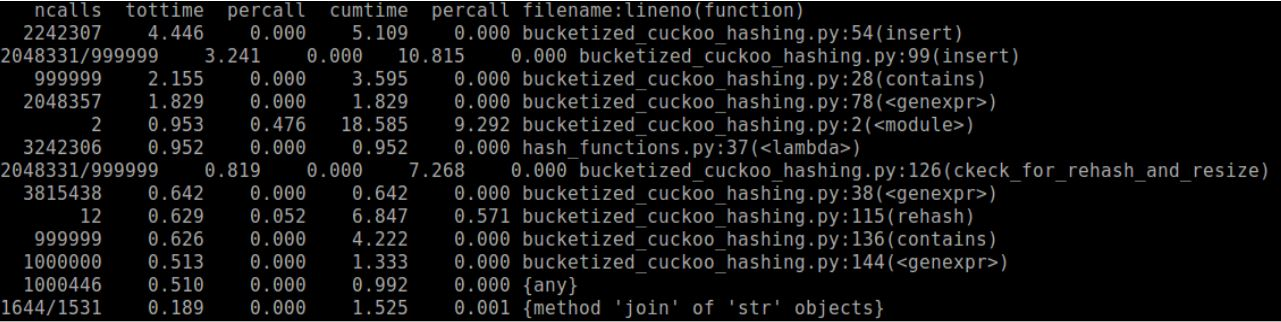
\includegraphics[width=1.0\textwidth]{Bilder/cprofiler.jpg}
	\caption{Analyse durch cProfile}
\end{figure}
Die Ausgabe gibts Auskunft darüber, wie oft bestimmte Funktionen aufgerufen wurden und wie viel Zeit bei deren Bearbeitung verbraucht wurde.

Mit Hilfe von \textit{cProfile} wurden Funktionen ausfindig gemacht, die unerwartet viel Laufzeit verbraucht haben. Um den Umfang der Dokumentation halbwegs in Grenzen zu halten, wird nun auf Optimierungen eingegangen, die im Lauf der Analyse mit \textit{cProfile} durchgeführt wurden.

\subsection{Berechnung mit den Hash-Funktionen}
Die Berechnung der Hash-Werte mit den universalen Hash-Funktion hat unerwartet viel Laufzeit gekostet. Wie bereits vorgeführt, haben die Hash-Funktionen die Form \(((a*x+b)\%p)\%m\), wobei \textit{x} das Argument ist, \textit{a} und \textit{b} zwei Zufallszahlen, \textit{p} eine Primzahl und \textit{m} die Größe der Hash-Tabelle.

Unter der Einschränkung, dass die Größen der Hash-Tabellen stets Zweierpotenzen sind, kann anstatt \(x\%m\) auch \(x\&(m-1)\) geschrieben werden. Dabei ist der Operator \textit{\&} das bitweise Und. Die Berechnung hat sich auf diese Weise als schneller herausgestellt. 

\subsection{Berechnung von Primzahlen}
Die Primzahl \textit{p}, die für die Hash-Funktionen generiert wird soll eine Primzahl sein, die größer als \textit{m} ist. Für das Generieren von Primzahlen wurden verschiedene Ansätze probiert. 

Generell ist es für das Generieren von großen Primzahlen üblich, eine Zufallszahl zu generieren und diese mit einem probabilistischen Primzahltest zu überprüfen. Die Primzahlen, die hier benötigt werden, liegen jedoch nicht in einer Größenordnung, wo sich diese Herangehensweise auszahlt.

Eine weitere Variante, die unerwarteterweise keine Erfolg erbracht hat, war, eine große Menge an bereits berechneten Primzahlen in einer Datei zu speichern und diese bei Bedarf auszulesen. Gleiches gilt für die Verwendung eines Siebs, wie zum Beispel das Sieb von Atkin.

\newpage
Letztendlich hat sich folgende Variante als guter Kompromiss herausgestellt:
\begin{lstlisting} [caption={Berechnung einer größeren Primzahl}]
def next_prime(n):
    p = n+1
    q = n*3
    for _ in xrange((q - p) ** 2 + 20):
        i = randint(p, q) | 1
        if is_prime(i):
            return i               
\end{lstlisting}
Dabei nutzt die Funktion \textit{is\_prime} die Eigenschaft aus, dass Primzahlen stets Nachbarn von Vielfachen der Zahl 6 sind und schränkt somit den Suchraum ein.

\subsection{Generatoren anstatt Listen}
Die \textit{List Comprehension} in Python berechnet direkt alle Elemente in der Liste. Nutzt man stattdessen Generatoren, werden die Elemente erst bei Bedarf ausgewertet. Der Unterschied macht sich vor Allem bemerkbar, wenn in Kombination Ausdrücke wie \textit{any} oder \textit{all} verwendet werden, wodurch in manchen Fällen Operationen eingespart werden können. Die Verwendung von Generatoren wird allgemein empfohlen, wenn die Daten lediglich einmal gebraucht werden. Ein Beispiel ist folgende Optimierung, die bei der Suche nach einem Schlüssel in einem Bucket durchgeführt wurde:
\begin{lstlisting} [caption={Generator und Any anstatt List Comprehension}]
#vorher
return len([curr for curr in bucket[1:bucket_index] if curr == key])
#nachher
return any((curr == key for curr in bucket[1:bucket_index]))         
\end{lstlisting}

\section{Implementierung des Kuckucks-Hashing mit Buckets}
In den Laufzeitmessungen des Kuckucks-Hashing hat sich herausgestellt, dass das Re-Hashing einen großen Einfluss auf die Laufzeit des Algorithmus hat. Beim Kuckucks-Hashing  wird jedes mal ein Re-Hashing durchgeführt, wenn der Füllgrad den Wert 0.5, da ab diesem Wert das Chance, dass beim Einfügen die maximalen Schleifendurchläufe erreicht werden, enorm ansteigt. 

Das Kuckucks-Hashing mit Buckets verfolgt das Ziel, einen Füllgrad von bis zu 1 zu unterstützen, wodurch weniger oft ein Re-Hashing durchgeführt werden muss. Dafür wird jedes Feld der Hash-Tabellen zu einem Bucket, also einem Array, welches hier Platz für vier Datensätze hat. Falls eine Vielzahl von Elementen beim Einfügen ein Re-Hashing hervorrufen gibt es noch die Optionen, diese Elemente stattdessen in einem Stash zu speichern. Der Stash ist dabei ein Array fester Größe, welches mit linearem Hashing und einer Modulo-Funktion betrieben wird. Die Implementierung wird vorerst ohne den Stash vorgenommen und mit dem normalen Kuckucks-Hashing verglichen.

Die Operationen des Kuckucks-Hashing selbst müssen kaum modifiziert werden. Jedoch gibt es eine neue Klasse \textit{BucketTable}, welche die beiden Hash-Tabellen darstellt und die entsprechenden Operationen \textit{insert} und \textit{contains} implementiert. Somit greift die eigentliche Klasse \textit{BucketizedCuckooHash} lediglich die Methoden von \textit{BucketTable} zu. Der Konstruktor für die Klasse \textit{BucketizedCuckooHash} ist folgender:
\begin{lstlisting} [caption={Konstruktur des Kuckucks-Hashing mit Buckets}]
class BucketizedCuckooHash(HashTable):
    def __init__(self, size):
        self.size = size
        self._elementcount = 0
        self._maxloop = int(log(size))
        self._table1 = BucketTable(size)
        self._table2 = BucketTable(size)                
\end{lstlisting}
Für die Implementierung ist vor Allem die bereits erwähnte Klasse \textit{BucketTable} interessant, deren Konstruktur wie folgt aussieht:
\begin{lstlisting} [caption={Konstruktur der einzelnen Hash-Tabellen mit Buckets}]
class BucketTable(object):
    def __init__(self, size):
        self.size = size
        self._table = size * [[]]
        self._hf = universal_hash(size)           
\end{lstlisting}
Ein Objekt \textit{BucketTable} stellt dabei eine Liste der Größe \textit{size} dar, dessen Felder Buckets sind. Die Buckets sind wiederum Listen der Länge 9, die Platz für vier Datensätze haben. Dabei gelten für die Felder der Buckets folgende Eigenschaften:
\begin{itemize}	
	\item die Felder bucket[1..4] enthalten Schlüssel
	\item die Felder bucket[5..8] enthalten Werte
	\item für \(i\in{1\dots{}4}\) gilt: der Wert bucket[i+4] gehört zum Schlüssel bucket[i]
	\item bucket[0] ist der Index, an dem der nächste Schlüssel einzufügen ist oder 5
\end{itemize}
Die \textit{insert}-Methode der Klasse \textit{BucketizedCuckooHash} ruft die \textit{insert}-Methode der Klasse \textit{BucketTable} mit einem einzufügenden Datensatz auf und erwartet als Rückgabewert den verdrängte Datensatz oder das Tupel (-1, -1) als Zeichen für ein kollisionsfreies Einfügen. Eine Kollision entsteht dabei, wenn ein Bucket bereits komplett befüllt ist. Dann wird der einzufügende Datensatz an der Position des ersten Datensatzes im Bucket eingefügt, welcher zum Rückgabewert der Methode wird. 

Falls die Hash-Tabellen zu viel Speicherplatz in Anspruch nehmen sollten, kann das erste Feld in den Buckets entfernt werden. Demnach wird beim einfügen durch den Bucket iteriert, bis ein freies Feld oder das Ende des Buckets erreicht wurden.
\newpage
Das Einfügen wurde folgendermaßen implementiert:
\begin{lstlisting} [caption={Implementierung des Einfügens in Hash-Tabellen mit Buckets}]
def insert(self, key, value):
    addr = self._hf(key)

    try:
        bucket = self._table[addr]
        bucket_index = bucket[0]
    except IndexError:
        bucket = self._table[addr] = [2, key, None, None, None, value, None, None, None]
        return -1, -1

    if bucket_index == 5:
        evicted_key = bucket[1]
        evicted_val = bucket[5]
        self._table[addr][1] = key
        self._table[addr][5] = value
        return evicted_key, evicted_val
    else:
        self._table[addr][bucket_index] = key
        self._table[addr][bucket_index + 4] = value
        self._table[addr][0] += 1
        return -1, -1      
\end{lstlisting}
Die Zeilen 7-9 bilden das Grundgerüst für einen neuen Bucket, falls auf diesen das erste mal zugegriffen wird.
\newpage
Wird die \textit{contains}-Operation aufgerufen, so muss zunächst der entsprechende Bucket ermittelt werden, in dem jeder Schlüssel mit dem gesuchten Schlüssel verglichen wird:
\begin{lstlisting} [caption={Implementierung des Suchens in Hash-Tabellen mit Buckets}]
def contains(self, key):
    addr = self._hf(key)

    try:
        bucket = self._table[addr]
        bucket_index = bucket[0]
    except IndexError:
        return False

    return any((curr == key for curr in bucket[1:bucket_index]))  
\end{lstlisting}
Ob sich der zusätzliche Implementierungsaufwand bezahlt gemacht hat und das Kuckucks-Hashing mit Buckets tatsächlich einen höheren Füllgrad erlaubt, sollen die Laufzeitmessungen zeigen.

\textit{Vergleich von Kuckucks-Hashing mit und ohne Buckets}
Zunächst wurden die Laufzeitmessungen mit synthetisierten Sequenzen aus MAC-Adressen aus Kapitel 3.2 für diese Implementierung durchgeführt. Nachfolgend sind die Diagramme der durchschnittlichen Laufzeiten im Vergleich in der Reihenfolge kleine, mittlere und große Netzwerke abgebildet.
\newpage\thispagestyle{empty}
\begin{figure}[H]
	\vspace*{-2.0cm}\hspace*{-1.7cm}\includegraphics[width=1.5\linewidth]{Bilder/vergleich_average.pdf}
\end{figure}
\newpage
Die Diagramme zeigen, dass die Implementierung des Kuckucks-Hashing mit Buckets anscheinend in alle untersuchten Fällen langsamer ist, als das Kuckucks-Hashing ohne Buckets. Die Entwicklung der Laufzeit ist ähnlich linear, jedoch ist der Anstieg höher. Was des Weiteren auffällt ist, dass sich die durchschnittlichen Laufzeiten für das Kuckucks-Hashing mit Buckets für die verschiedenen Testfälle kaum verändern, während die Laufzeiten des Kuckucks-Hashing ohne Buckets im Schnitt ansteigen. Auf Basis dieser Beobachtung lässt sich die Vermutung anstellen, dass mit steigender Anzahl der disjunkten MAC-Adressen in den Eingabedaten ab einem gewissen Punkt die Implementierung mit Buckets schneller wird, als die Implementierung ohne. Diese Vermutung Bedarf jedoch genauerer Nachmessungen und ist für das gewünschte Anwendungsszenario weniger relevant. Die Messergebnisse deuten an, dass das Kuckucks-Hashing ohne Buckets für die Analyse von pcap-Dateien besser geeignet ist.

\section{Hypothesentest}
Die Annahme ist, dass Kuckucks-Hashing in den Messungen schneller war als Kuckucks-Hashing mit Buckets. Demnach ist die Null-Hypothese \(H_{0}: \tilde{\mu}_{1} \ge \tilde{\mu}_{2} \), wenn \(\mu_{2}\) die Mittelwerte der Messungen für Kuckucks-Hashing und \(\mu_{1}\) für Kuckucks-Hashing mit Buckets sind. Daraus ergeben sich für die drei Testfälle folgende Werte:
\begin{table}[H]
	\centering
	\begin{tabular}{|c|c|c|}
		\hline
		Testfall & \(\mu_{d}\) & \(\delta_{d}\) \\ \hline
		small & 6,974024985 & 3,31504764506 \\
		medium & 7,6520616212 & 3,57926752039 \\
		large & 4,947120686 & 3,66159999932 \\ \hline
	\end{tabular}
	\caption{Berechnung von \(\mu_{d}\) und \(\delta_{d}\)}
\end{table}
Dabei ist \(\mu_{d}\) der Durchschnitt aus der Differenz aller durchschnittlichen Laufzeiten von Kuckucks-Hashing mit und ohne Buckets und \(\delta_{d}\) die Standardabweichung. Aus diesen Werten lässt sich der Wert \textit{t} mit \(t=\sqrt{5}*(\mu_{d}-0)/\delta_{d}\) bilden, woraus folgt:
\begin{table}[H]
	\centering
	\begin{tabular}{|c|c|}
		\hline
		Testfall & \textit{t} \\ \hline
		small & 4,704  \\
		medium & 4,7805  \\
		large & 3,0211  \\ \hline
	\end{tabular}
	\caption{Berechnung von \textit{t}}
\end{table}
Für ein Signifikanzniveau \(\alpha_{1} = 0.995\) gilt \(t_{1}(0,995, 4) \approx 4.604\) und für \(\alpha_{2} = 0.975\) gilt \(t_{2}(0,975, 4) \approx 2.776\). Für die Testfälle small und medium lässt sich demnach mit \(\alpha_{1}\) die Nullhypothese ablehnen, da \(t < t_{1}(\alpha_{1}, 4)\). Das heißt, dass Kuckucks-Hashing mit einer Irrtumswahrscheinlichkeit von \(0.05\) schneller war als das Kuckucks-Hashing ohne Buckets. Gleiches gilt für den Testfall large, jedoch mit einer Irrtumswahrscheinlichkeit von \(0.25\).